\chapter{Methodology}
\label{chap:methodology}

\section{System Design Approach}
Lectura was designed following modern cloud-native architectural principles. The architecture separates the application into two main layers: a client-side React frontend and a concurrent Go-based backend. This separation of concerns keeps the user interface responsive even when the backend is busy processing AI generation requests, which can take considerable time. The frontend handles client-side state management independently, while the backend focuses on data persistence, API coordination, and asynchronous job processing.

A ``web-first'' approach was chosen instead of building separate native mobile or desktop applications. This decision aligns with the typical usage patterns of the target audience: university students primarily use laptops for content consumption, lecture viewing, and research. To maintain usability on smaller screens — for example, reviewing flashcards on a phone during a commute — the interface uses Tailwind CSS with breakpoint-driven responsive layouts.

\section{AI Prompt Engineering Strategy}
When working with large language models, prompt engineering becomes a core part of the system architecture rather than an afterthought. The Lectura backend takes the cleaned input data and runs it through a multi-stage prompting pipeline:

\begin{itemize}[label=\textendash]
    \item Hierarchical Summarization: When the input exceeds 15,000 tokens, a single prompt tends to suffer from ``lost in the middle'' degradation, where the model ignores content in the middle of long inputs. Lectura handles this by splitting the text into overlapping chunks, summarizing each one separately, and then running a second ``meta-prompt'' that combines these partial summaries into a single coherent output.
    \item Bloom's Taxonomy Quiz Generation: The quiz generation prompts are structured around Bloom's Taxonomy. Instead of producing simple recall-based questions, the prompts instruct the model to generate higher-order questions that require analysis, application, and synthesis of concepts.
    \item Flashcard Generation: Flashcard prompts use strict formatting constraints that force the model to break down complex topics into short, focused question-answer pairs. Each card targets a single concept, and the prompts occasionally include instructions to add mnemonic hints for particularly difficult definitions.
    \item Chain-of-Thought (CoT) Prompting: For dense technical or mathematical content, the backend includes a Chain-of-Thought instruction (e.g., ``Before writing the final summary, list the key concepts in order...''). This makes the model show its reasoning steps before producing the final output, which reduces the chance of hallucinated content.
\end{itemize}

These prompt structures directly address Objective 3, Objective 5, and Objective 6 from the Introduction, covering the generation of summaries, quizzes, and flashcards respectively.

\section{Worker Pool Architecture and Asynchronous Processing}
Processing a two-hour lecture — generating summaries, a quiz, and a flashcard deck — typically takes between 10 and 60 seconds due to LLM response times. If this processing were handled synchronously within a standard HTTP request, users would experience connection timeouts and unresponsive browser tabs, likely causing them to leave the page.

To avoid this, Lectura uses a Worker Pool pattern. When a user submits content for processing, the backend creates a ``Job Ticket'' in the database queue and immediately returns a \texttt{202 Accepted} response to the frontend. In the background, a pool of Go goroutines monitors the queue. When a worker picks up a job, it handles the Gemini API calls, parses the responses, and stores the finished artifacts in the database. The workers also implement Exponential Backoff retries to handle API rate limits from external providers.

\subsection{Concurrency Model: Goroutines vs. OS Threads}
The choice of Go as the backend language was motivated largely by its M:N goroutine scheduler, which differs significantly from traditional 1:1 OS threading models. In a conventional application (e.g., Python or older Java frameworks), each concurrent task requires an OS thread with a stack allocation of roughly 1--2 Megabytes (MB). If 10,000 students were to request content generation at the same time, the server would need approximately 20 GB of RAM just for thread stacks — enough to cause Out-Of-Memory (OOM) crashes before any real work begins.

Go goroutines, by contrast, start with a stack of approximately 2 Kilobytes (KB). The Go runtime maps many goroutines onto a smaller number of OS threads. When a goroutine blocks on an HTTP request to the Gemini API, the scheduler moves it off the OS thread and replaces it with another ready goroutine in $O(1)$ time, without requiring a full kernel-level context switch.

The memory required for concurrent connections scales as follows:

\begin{equation}
    \text{Mem}_{\text{traditional}} = N \times (2 \cdot 10^6 \text{ Bytes}) \gg \text{Mem}_{\text{Go}} = N \times (2 \cdot 10^3 \text{ Bytes})
\end{equation}

This roughly 1000x reduction in per-connection memory cost allows Lectura to handle traffic spikes during exam periods without requiring expensive cloud infrastructure. This concurrency model directly addresses Objective 10, providing the resilience needed to handle slow LLM API responses without blocking the main server thread.

\section{WebSocket Real-Time Updates}
Since the content generation happens in background workers, the React frontend needs a way to receive progress updates in real time. Instead of polling the server repeatedly with REST requests, Lectura uses WebSockets for bidirectional communication.

When a user submits a generation request, the React client opens a persistent WebSocket connection to the backend \texttt{/ws} endpoint, authenticating with a JWT token. As the background worker progresses through the job, it pushes status updates through this channel — events like \texttt{JOB\_QUEUED}, \texttt{TRANSCRIPT\_SANITIZED}, \texttt{SUMMARY\_GENERATING}, and \texttt{GENERATION\_COMPLETE}. Heartbeat pings and automatic reconnection logic ensure the connection recovers from temporary network interruptions.

\subsection{WebSocket vs. HTTP Polling Overhead}
Using WebSockets avoids the significant overhead of repeated HTTP polling. Each HTTP/1.1 request includes headers (User-Agent, Cookie, Accept-Encoding, etc.) that typically add 700 to 1200 bytes per request. If the frontend polled a \texttt{/status} endpoint every 2 seconds across 1,000 active users, the server would handle over 1.2 MB/s of traffic consisting entirely of redundant headers.

With the RFC 6455 WebSocket protocol, after the initial \texttt{HTTP/1.1 101 Switching Protocols} handshake, subsequent data frames carry only a small 2-to-10 byte framing header. This reduces the bandwidth used for status updates by roughly 98\%, freeing network capacity for the actual transfer of generated content.

\section{Database Schema Design}
The PostgreSQL schema was designed to balance relational integrity with the flexibility needed for AI-generated content. User accounts, authentication data, and session information are normalized to Third Normal Form (3NF) to prevent data redundancy. Indexes on the \texttt{user\_id} and \texttt{created\_at} columns speed up common queries, particularly when loading the dashboard and content library.

The artifacts produced by the LLM — such as arrays of quiz questions or structured summary JSON — are stored using PostgreSQL's native JSONB column type. This hybrid approach gives the team flexibility to update prompt formats without requiring database migrations, while still supporting efficient queries through JSONB indexing.

\section{Interactive State Management and Inline Editing}
While the Go backend handles the initial content generation, the React frontend manages the editing of those generated artifacts. In particular, the presentation feature treats generated slides not as static outputs, but as editable documents.

The frontend uses a \texttt{SlideViewer} component that maintains the slide data as a nested JSON state. An \texttt{EditableText} component allows inline editing: when a user clicks on a slide heading, the static \verb|<h2/>| element is replaced with an auto-resizing \verb|<textarea/>|, providing a WYSIWYG-like editing experience.

To avoid sending a separate HTTP PUT request for every keystroke, the application uses a debounce mechanism. The debounce hook waits for a set interval (e.g., 1000ms) after the last keystroke before sending the updated content to the backend. If the user types again within that window, the timer resets. This ensures that edits are persisted reliably without creating unnecessary network traffic. The flow is illustrated in Figure~\ref{fig:debounce_flow}. This editing capability directly addresses Objective 4, which required a presentation engine with inline editing support.

\begin{figure}[htbp]
\centering
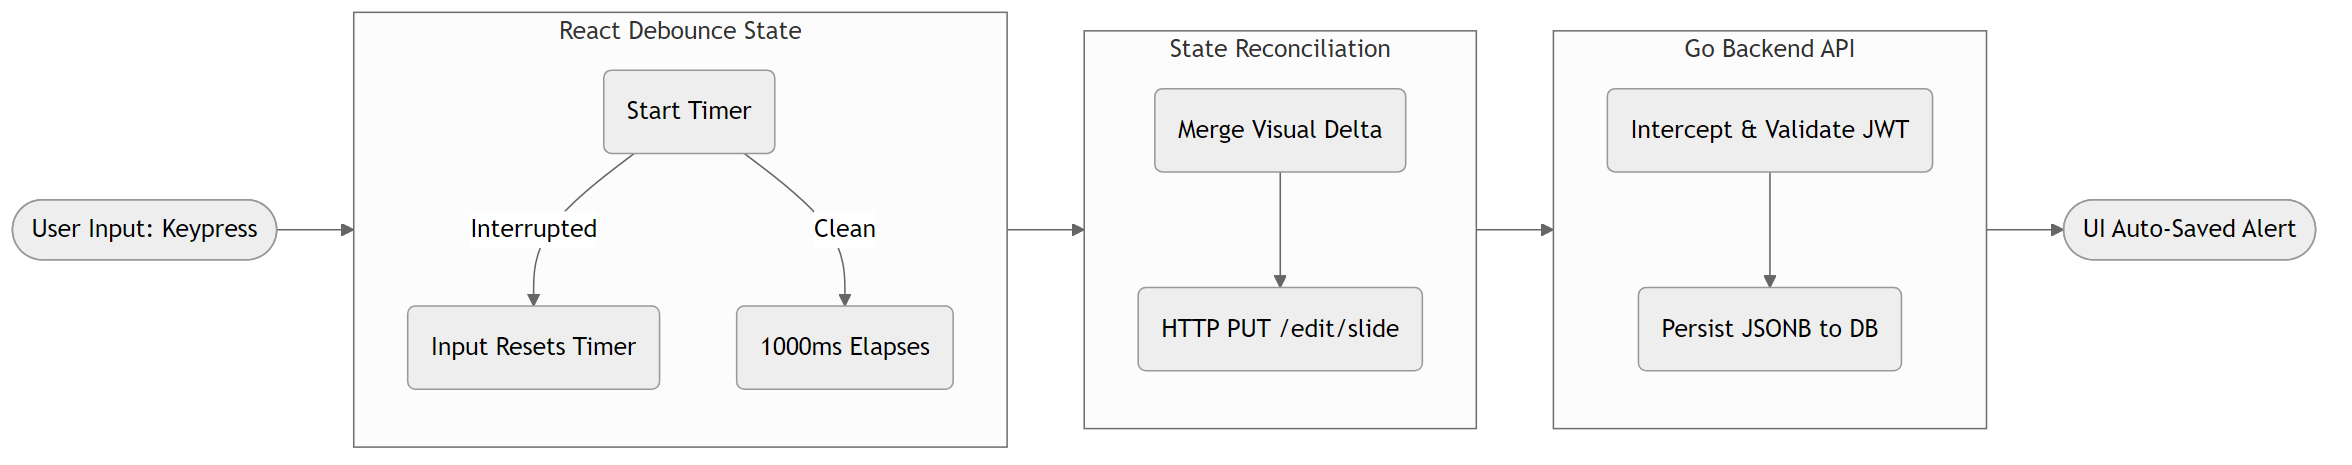
\includegraphics[width=\textwidth]{chapters/chapter04/images1/debounce.png}
\caption{State flow diagram for the Presentation Inline Editor debounce mechanism.}
\label{fig:debounce_flow}
\end{figure}

\section{Security Implementation}
Security is an important consideration for any web application handling user data. Lectura uses JWT (JSON Web Token) authentication with short-lived access tokens (15-minute expiry) and longer-lived refresh tokens tied to specific cryptographic keys.

Cross-Origin Resource Sharing (CORS) policies restrict which domains can interact with the API. All database queries use parameterized statements to prevent SQL injection. Both AI-generated outputs and user-submitted text are sanitized on the server side to prevent Cross-Site Scripting (XSS) attacks before being stored or displayed. Rate limiting on authentication endpoints protects against brute-force login attempts and denial-of-service attacks. These security measures support the data integrity requirements of Objective 8, ensuring that user analytics and session data remain protected.

\section{Subscription Management and Payment Integration}
To support the ongoing costs of running Large Language Models, Lectura includes a tiered subscription system. Processing long transcripts through models like Google Gemini requires computing resources, which makes a completely free service difficult to maintain long-term. To address this, a payment integration was implemented using Stripe.

\subsection{Tiered Access Model}
The platform uses a freemium model. Users start on a free tier, which allows them to test the core features of the platform with a limited number of generations per month. For users who need to process more lectures, premium tiers are available. These paid plans increase the monthly generation limits and provide access to more resource-intensive features. This structure helps balance the API costs by ensuring that heavy users contribute to the operating expenses.

\subsection{Stripe Checkout and Webhook Architecture}
The payment processing is handled entirely by the backend using the Stripe Go SDK (\texttt{stripe-go/v78}). When a user decides to upgrade their plan, the server calls the \texttt{CreateCheckoutSession} method. This generates a secure payment link hosted by Stripe. The user completes the transaction on Stripe's website, which means Lectura does not need to store or process sensitive credit card information locally.

After a successful payment, Stripe sends a webhook event (\texttt{checkout.session.completed}) back to the Lectura server. To ensure the request is legitimate, the \texttt{ConstructWebhookEvent} method checks the cryptographic signature using a secret key. Once verified, the backend reads the \texttt{user\_id} attached to the session and updates the user's subscription status in the PostgreSQL database.

Users can also manage their subscriptions through a Billing Portal. By calling the \texttt{CreateBillingPortalSession} method, the system redirects users to a self-service page where they can update their payment methods or cancel their plan without needing to contact an administrator.

\subsection{Security Considerations}
Using a third-party service like Stripe simplifies compliance with financial security standards like PCI DSS. Because the payment forms are hosted by Stripe, cardholder data never touches the Lectura frontend or backend servers. Additionally, all API keys and webhook secrets are stored securely in environment variables, protecting the payment infrastructure from unauthorized access.